\section{Experiment}
We applied this search strategy to dataset generated by the classic lamination
theory and failure theories. In this dataset, sixtheen attribues and two actual
values are given.

\subsection{Dataset Preparation}
Equation \ref{equ:stress-strain} takes an analytical approach to model the
relationship between stress and strain. We sample this function to yield 14000 points
uniformly distributed over the domain space.

The range of in-plane loading is from 0 to 120; the range of fiber orientation $\theta$ is from
-90 to 90; ply thickness $t$ is 1.27mm, number of plies range $N$ is from 4 to 120;
Three different material is used in this experiment, as shown in table \ref{tab:mat}.
Figure \ref{tab:traing-data} shows part of the training data.

In order to speeds up the learning and accerlate convergence, the input
atttributes of the data set are rescaled to between 0 and 1.0 by a linear function.

\begin{table}	
\label{tab:traing-data}
		\resizebox{\textwidth}{!}{
	\begin{tabular}{cccc|cc}
		\toprule
		\multicolumn{4}{c}{\textbf{Input}} &  \multicolumn{2}{c}{\textbf{Output}} \\
		\midrule
		Load  &  \makecell{Laminate \\ Structure }  & \makecell{Material \\ Property} & \makecell{Failure \\  Property}  & MS & Tsai-Wu \\
		\midrule

		-70,-10,-40,  & 90,-90,4,1.27, & 38.6,8.27,0.26,4.14,  & 1062.0,610.0,31,118,72,  & 0.0102, & 0.0086 \\
		-10,10,0,     & -86,86,80,1.27,& 181.0,10.3,0.28,7.17, & 1500.0,1500.0,40,246,68, & 0.4026, & 2.5120 \\
		-70,-50,80,   & -38,38,4,1.27, & 116.6,7.67,0.27,4.173,& 2062.0,1701.0,70,240,105,& 0.0080, & 0.0325 \\
		-70,80,-40,   & 90,-90,48,1.27,& 38.6,8.27,0.26,4.14,  & 1062.0,610.0,31,118,72,  & 0.0218, & 0.1028 \\
		-20,-30,0,    & -86,86,60,1.27,& 181.0,10.3,0.28,7.17, & 1500.0,1500.0,40,246,68, & 0.6481, & 0.9512 \\
		0,-40,0,      & 74,-74,168,1.27,& 181.0,10.3,0.28,7.17,& 1500.0,1500.0,40,246,68, & 1.3110, & 3.9619 \\
		\bottomrule
		\end{tabular}
	}
\end{table}

\begin{table*}[ht]
\caption{Comparison of the carbon/epoxy, graphite/epoxy, and glass/epoxy properties}
\centering
\begin{adjustbox}{width=1\textwidth}
\label{tab:mat}
\begin{tabular}{cccccc}
\toprule
Property								   & Symbol				  & Unit  &  Carbon/Epoxy&  Graphite/Epoxy  &  Glass/Epoxy   \\
\midrule
Longitudinal elastic modulus			   & $E_1$				  & GPa   &  116.6       &  181             &  38.6           \\
Traverse elastic modulus				   & $E_2$				  & GPa   &  7.67        &  10.3            &  8.27           \\
Major Poisson's ratio					   & $v_{12}$			  &       &  0.27        &  0.28            &  0.26           \\
Shear modulus							   & $G_{12}$			  & GPa   &  4.17        &  7.17            &  4.14           \\
Ultimate longitudinal tensile strength     & $(\sigma_1^T)_{ult}$ & MP    &  2062        &  1500            &  1062            \\
Ultimate longitudinal compressive strength & $(\sigma_1^C)_{ult}$ & MP    &  1701        &  1500            &  610             \\
Ultimate transverse tensile strength       & $(\sigma_2^T)_{ult}$ & MPa   &  70          &  40              &  31              \\
Ultimate transverse compressive strength   & $(\sigma_2^C)_{ult}$ & MPa   &  240         &  246             &  118              \\
Ultimate in-plane shear strength           & $(\tau_{12})_{ult}$  & MPa   &  105         &  68              &  72               \\
Density                                    & $\rho$               & $g/cm^3$ &  1.605    &  1.590           &  1.903               \\
Cost                                       &                      &       &  8           &  2.5             &  1               \\
\bottomrule
\end{tabular}
\end{adjustbox}
\end{table*}


\begin{figure}[h!]
	\centering
	\begin{subfigure}[b]{1.0\linewidth}
		\centering
		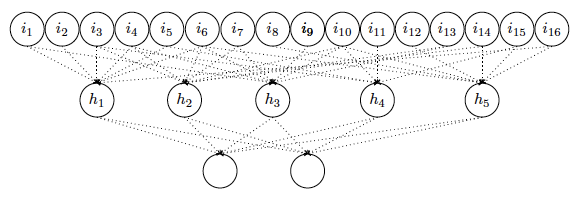
\includegraphics[width=0.8\textwidth]{./a0_figure_ann_for_clt_architecture_example1.png}
		\caption{Parent 1}
		\label{fig:p1}
	\end{subfigure}
	\newline
	\begin{subfigure}[b]{1.0\linewidth}
		\centering
		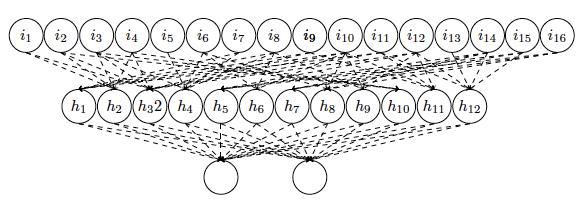
\includegraphics[width=0.8\textwidth]{./a0_figure_ann_for_clt_architecture_example2.png}
		\caption{Parent 2}
		\label{fig:p2}
	\end{subfigure}
	\newline
	\begin{subfigure}[b]{1.0\linewidth}
		\centering
		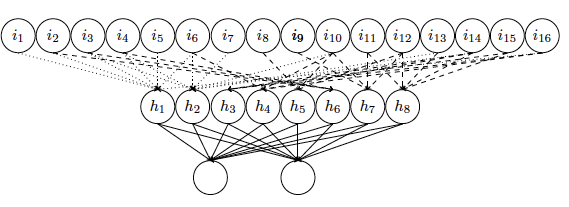
\includegraphics[width=0.8\textwidth]{./a0_figure_ann_for_clt_architecture_child.png}
		\caption{Child}
		\label{fig:child}
	\end{subfigure}
	\caption{Search Operation}
	\label{fig:search}
\end{figure}
